
\documentclass[12pt]{article}
%	options include 12pt or 11pt or 10pt
%	classes include article, report, book, letter, thesis

\title{Scalable Mixed-Integer Path Planning for UAVs}
\usepackage{amsmath}
\usepackage{relsize}
\usepackage{mathtools}
\usepackage{graphicx}
\usepackage{caption}
\usepackage{subcaption}
\usepackage{hyperref}
\author{Jorik De Waen}
\date{\today}

\begin{document}
\maketitle

\section{Introduction}
Path planning is currently an unsolved problem for unmanned drones. Even though most modern quadrocopters are capable of flying by themselves, they are unable to generate a flight path that will get them to their destination reliably. Classic graph-based shortest path algorithms like Dijkstra's algorithm its many variants fail to take momentum and other factors into account. Mixed Integer Linear Programming (MILP) is one approach that shows promising results, however it is currently severely limited by computational complexity.


\subsection{Motivation}
One of the main advantages of using a constraint optimization approach like MILP is that they are extremely extendable by design. A system based on this can be deployed in many different scenarios with different goals and constraints without the need for significant changes to the algorithms that drive it. The solvers that construct the final path are general solvers which take constraints and a target function as input. This input can be generated by end users in the field to match their specific requirements, making the software controlling the drones as flexible as the hardware.
\par
That flexibility is also the main limitation of using constraint optimization. The solvers are general purpose, which make them very slow compared to more direct approaches. They need to be carefully guided solve all but the most basic scenarios in a reasonable amount of time. While there have been some good results on small scales, I could not find any attempts at planning paths on the order of kilometers or more. Practical use cases involving drones often involve several minutes of flight and can cover several kilometers, so a path planner must be able to work at such a scale. This is the main goal of the thesis: To demonstrate how a MILP approach can be scaled to scenarios with a much larger scope, while preserving the advantages that make it interesting.

\subsection{Context}
\label{subsec:previous}
Mixed integer linear programming is and extension of linear programming. In a linear programming problem, there is a single (linear) target function which needs to be minimized or maximized by the solver. A problem typically also contains a number linear inequalities which constrain the values of the variables in the target function.
\begin{figure}[h]
\begin{math}
\text{maximize} \quad 100 x_1 + 125 x_2 \\
\text{subject to} \\
3 x_1 + 6 x_2 \leq 30 \\
8 x_1 + 4 x_2 \leq 44
\end{math}
\caption{An example linear problem}
\end{figure}
When all the variables are real, problems like this can be solved in polynomial time. However, only convex search spaces can be modeled this way. By adding obstacles to the world the drone has to navigate, the search space becomes non-convex. To express non-convex search spaces, integer variables are required\cite{Schouwenaars2001}. A linear problem with integer variables is called a mixed integer linear problem. These integers make it possible to model logical expressions, which in turn enable approximations of non-linear function to be used. Another consideration is how to model time. Constraint solvers typically have no concept of time, so this needs to be modeled as well. \\
The most common way to do this is the way Schouwenaars et al\cite{Schouwenaars2001} originally modeled time: A limited amount of discrete timesteps. Planning using MILP is very computationally expensive, so an attempt by Bellingham\cite{Bellingham2002} was to use a receding horizon and only plan a small part of the path at a time. \\ 
Flores\cite{Flores2007} and Deits et al\cite{Deits2015} do not use discretized time, but model continuous curves instead. This no longer uses linear programming, but quadratic, conic or higher.
\\
Several different papers\cite{Fliess1995a, Hao2005, Cowling2007, Mellinger2011} show how the output from algorithms like these can be translated to control input for an actual physical vehicle. This demonstrates that, when they properly model a vehicle, these path planners need minimal post-processing to control a vehicle.
\section{Modeling Path Planning as a MILP problem}
\label{section:modeling}
The path planning problem can be represented with discrete timesteps with a set of state variables for each epoch. The amount of timesteps determines the maximum amount of time the vehicle has in solution space to reach its goal. The actual movement of the vehicle is modeled by calculating the accelleration, velocity and position at each timestep based on the throttle (in each axis) and state variables from the previous time step.

\begin{figure}[h]
\begin{math}
time_0 = 0 \\
time_{t+1} = time_{t} + \Delta t,  \quad 0 \leq t < N \\ \\
\boldsymbol{pos}_0 = \boldsymbol{pos}_{start} \\
\boldsymbol{pos}_{t+1} = \boldsymbol{pos}_{t} + \Delta t * \boldsymbol{vel}_{t}  \quad 0 \leq t < N \\ \\
\boldsymbol{vel}_0 =\boldsymbol{vel}_{start} \\
\boldsymbol{vel}_{t+1} =\boldsymbol{vel}_{t} + \Delta t * \boldsymbol{acc}_{t}  \quad 0 \leq t < N \\ \\
\boldsymbol{acc}_{t} = \boldsymbol{throttle}_{t} * \boldsymbol{acc}_{max}  \quad 0 \leq t \leq N \\
\end{math}
\end{figure}

The problem also needs a goal function to optimize. In this model, the goal is to minimize the time before a goal position is reached. Optionally, there is also a goal velocity that needs to be matched when the vehicle reaches the goal. Reaching the goal constraints causes a state transition from not being finished to being finished. Modeling state transitions directly can be error-prone, so Lamport's\cite{Lamport1989} state transition axiom method was used. In this simple model it is still possible to model the state transition directly, but the goal of the thesis is to provide a flexible and extensible approach.


\begin{figure}[h]
\begin{math}
minimize \quad N - \mathlarger{\sum}_{t=0}^{t \leq N} fin_t \\
fin_0 = 1 \\ 
fin_{t+1} = fin_t \vee cfin_{t+1},  \quad 0 \leq t < N \\ \\
cfin_{pos,t} =  \mathlarger{\mathlarger{\bigwedge_{i = 0}^{i < Dim(\boldsymbol{pos}_t)}}} |pos_{t,i} - pos_{goal, i}| < pos_{tol},  \quad 0 \leq t \leq N \\ \\ \\
cfin_{vel,t} = 
\begin{cases*}
\mathlarger{\bigwedge_{i = 0}^{i < Dim(\boldsymbol{vel}_t)}} |vel_{t,i} -vel_{goal, i}| < vel_{tol}& if $\boldsymbol{vel}_{goal}$ exists, $0 \leq t \leq N$  \\
true & otherwise, $0 \leq t \leq N$ 
\end{cases*} \\ \\ \\
cfin_t =  cfin_{pos,t} \bigwedge cfin_{vel,t} \quad 0 \leq t \leq N
\end{math}
\end{figure}

Vehicles have a maximum velocity they can achieve. Calculating the velocity of the vehicle means applying Pythagoras' theorem on the axis of the velocity vector. This is not possible using only linear equations. However, it can be approximated to an arbitrary degree using multiple linear constraints. The components of the velocity vector can be positive or negative, but only the absolute value matters for the actual velocity. 
\begin{figure}[h]
ABS \\
MAXSPEED
\end{figure}

The most challenging part of the problem is modeling obstacles. Any obstacle between the vehicle and its goal will inherently make the search space non-convex. Because of this, integer variables are needed to model obstacles. The most common way to do this is to use the ``Big M'' method to model a polygon. The size of the vehicle needs to be taken into account. Assuming the polygon is convex and the vertices of the polygon are listed in counter-clockwise order, the following constraints model an obstacle:

\begin{figure}[h]
OBSTACLE CONSTRAINTS \\
\end{figure}

Because obstacles make the problem non-convex and thus require integer constraints to model, the execution time scales very poorly with the amount of obstacles. This can be mitigated by only modeling a certain amount of obstacles relatively close to the vehicle, while limiting the vehicle to a convex region which does not overlap any of the ignored obstacles. Modeling this convex allowed region is very similar to modeling the obstacles, except that this time no integer variables are needed.

\begin{figure}[h]
ACTIVE REGION\\
\end{figure}

\section{Segmentation of the MILP problem}
\label{section:segment}

Short paths can be solved directly, but longer paths with a large amount of obstacles nearby take an extremely long time to solve. A solution to this problem is to divide the path into smaller segments. Solving the smaller segments is proportionally disproportionately easier than solving the full path, but at the cost of optimality and stability.
\\
\subsection{Finding the initial path}
The first issue is that because the goal cannot be reached immediately, the goal function needs to change.  \\
One option is to simply get as close as possible to the goal during each segment. Because the distance that can be traveled during a segment is limited, the amount of obstacles that need to be modeled is also limited. This works well when the world is very open with little obstacles. However, this greedy approach is prone to getting stuck in dead ends in more dense worlds like cities.
\\
The second option is finding a complete path using a method that's easier to compute. An algorithm like A* can be used to find a rough estimation for the path. This A* path is the shortest path, but does not take constraints or the characteristics of the vehicle into account. A very curvy direct path may be the shortest, but a detour which is mostly straight and allows for higher speeds may actually be faster. 
\\
It is possible to use more advanced algorithms that model more of the constraints. This will significantly improve the speed and quality of the constraint optimization step, but it will also come at a performance cost. A balance needs to be found between the preprocessing step and the constraint optimization step. The preprocessing step needs to do just enough so the optimization step can be solved in an acceptable amount of time. 
\\
I have decided to use Theta*. This is a variant  of A* that allows for paths at arbitrary angles instead of multiples of 45 degrees. The main reason for this is that it eliminates the ``zig zags'' that A* produces. This makes the next step of the preprocessing much easier.\\
\subsection{Detecting corner events}
With an initial path generated, the next problem is dividing it into segments. Dividing the path into equal parts presents problems, because when solving each segment, the solver has no knowledge of what will happen in the next segment. This is especially problematic when the vehicle needs to make a tight corner. If the last segment ends right before the corner, it may not be possible to avoid a collision.\\
In Euclidian geometry, the shortest path between two points is always a straight line. When polygonal obstacles are introduced between those points, the shortest path will be composed of straight lines with turns at one or more vertices of the obstacles. The obstacle that causes the turn will always be on the inside of the corner. This shows why corners are important for another reason: They make the search space non-convex. For obstacles on the outside of the corner it is possible to constrain the search space so it is still convex, but this is not possible for obstacles on the inside.\\
Because of these reasons, isolating the corners from the rest of the path is advantageous. With enough buffer before the corner, the vehicle is much more likely to be able to navigate the corner successfully. It also means that the computationally expensive parts of the path are as small as possible while still containing enough information for fast navigation through the corner.
\\
The reason for using Theta* becomes clear now. Every single node in the path generated by the algorithm is guaranteed to be either the start, goal or near a corner. A corner can have more than one node, so nodes which turn in the same direction and are close to each other are merged into a single corner event. A corner event is also generated for nodes which are alone.
\subsection{Generating path segments}
These corner events are in turn grown outwards to cover the approach and departure from the corner. How much depends on the maximum acceleration of the vehicle. As a rule of thumb: If the vehicle can come to a complete stop from its maximum speed before the corner, it can also successfully navigate that corner. When corners appear in quick succession, their expanded regions may overlap. In that case, the middle between those corners is chosen. Long, straight sections are also divided into smaller path segments.\\
One of the main goals of segmenting the path is to reduce the amount of obstacles. This means that every segment has a set of obstacles associated with it, being the obstacles that need to be modeled in the optimization step. Not only the obstacle that ``causes'' the corner is important, but obstacles which are nearby are important as well. Obstacles on the outside of the corner also may play a role in how the vehicle approaches the corner. To find all potentially relevant obstacles, the convex hull of the (Theta*) path segment is calculated and scaled up slightly. Every obstacle which overlaps with this shape is considered an active obstacle for that path segment. The convex hull step ensures that all obstacles on the inside of the corner are included, while scaling it up will cover any restricting obstacle on the outside of the corner.
\subsection{Generating the active region for each segment}
Even though the most important obstacles are taken care of, all other obstacles also need to be represented. To do this, a convex polygon is grown around the path. This polygon may intersect with the active obstacles (since they will be represented separately), but may not intersect any other obstacle. The polygon is grown using a genetic algorithm. It uses a single mutator which nudges the vertices of the polygon while ensuring it stays convex and does not intersect itself or any non-active obstacle. The genetic algorithm is just one way to generate the convex polygon which represents the active region. Deits and Tedrake\cite{Deits2015} have demonstrated how another algorithm can solve the same problem.
\section{Results}
One of the test scenarios used during development of the algorithm is the navigation through a 1km by 1km square section of the city of Leuven, Belgium. This data is freely available from the local government \footnote{\url{https://overheid.vlaanderen.be/producten-diensten/basiskaart-vlaanderen-grb}} and represents a real life scenario. Not all of the buildings in the dataset have a convex shape. The algorithm only handles convex obstacles, so the convex hull of each building is used. This area contains 3079 distinct buildings, ranging between 4 and well over 10 vertices per building. The path that needs to be planned is about 1.3km long. Figure \ref{fig:example} shows a visualization of the path and many other elements that go into calculating it.
\\
The grid size for Theta* is set at 5m, yielding a 200 by 200 grid. Calculating the initial path takes around 30 seconds. From this path, 21 segments are constructed. Each segments takes on average just under 11 seconds to solve, although the time to solve each segment ranges from 0.3s to 74s. The final path consists of 960 distinct timesteps at 10Hz, although significantly more have been calculated to ensure the vehicle can reach its goal in each segment within the given amount of timesteps for that segment.
\begin{figure}[h]
    \centering


    \begin{subfigure}[b]{0.6\textwidth}
        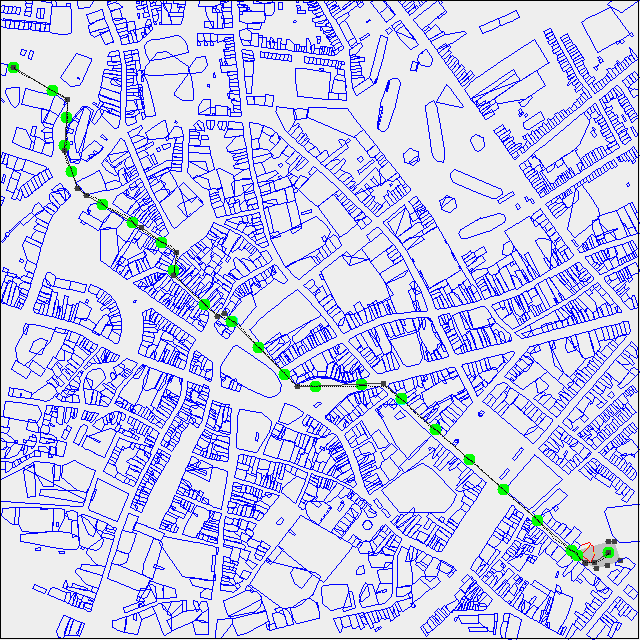
\includegraphics[width=\textwidth]{img/leuven}
    \end{subfigure}
        ~ %add desired spacing between images, e. g. ~, \quad, \qquad, \hfill etc. 
      %(or a blank line to force the subfigure onto a new line)
        \begin{subfigure}[b]{0.35\textwidth}
        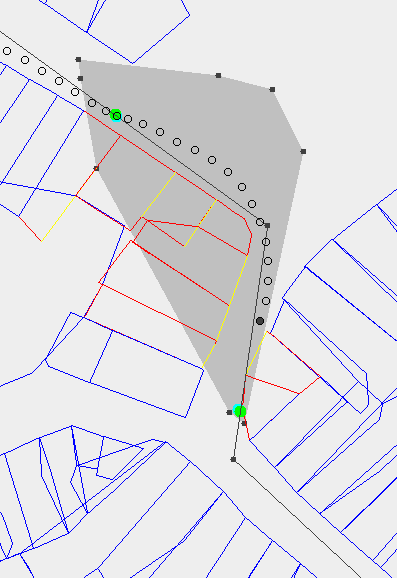
\includegraphics[width=\textwidth]{img/zoomed}
    \end{subfigure}
    \caption{The left image shows an overview of the 1km by 1km map, and the path from the top-left to the bottom-right. The right image shows a zoomed-in view of a part of the path. The blue polygons are buildings. The black segmented line is the initial Theta* path. The filled green circles represent the transitions between segments. The dark gray region on the right shows the active region, with the active obstacles in red and yellow. The current position of the vehicle is represented by the filled gray circle, while its position in the timesteps leading up to the current timestep are represented by the hollow gray circles.}\label{fig:example}
\end{figure}
\\
MILP path planning has not been demonstrated on a scale like this before. This technique can also scale even further. Given an initial path, the complexity of the algorithm scales roughly linearly with the amount of segments. The main bottleneck that prevents this approach from scaling up further is the Theta* step. By replacing Theta* with a more efficient implementation, or an entirely different algorithm, larger scales can be achieved.

\newpage
\bibliographystyle{plain}
\bibliography{../papers/bib.bib}
\end{document}